\documentclass[runningheads]{llncs}
\usepackage[T1]{fontenc}
\usepackage{graphicx}
\usepackage{amsmath,amssymb}
\usepackage{booktabs}
\usepackage{xcolor}
\usepackage{tikz}
\usetikzlibrary{arrows.meta,positioning}
\usepackage[hidelinks]{hyperref}
\graphicspath{{figures/}}

% Result macros: every reported number lives in results_macros.tex, regenerated from the experiment
% output by scripts/fill_paper_results.py (outputs/experiment/results.json). \na marks a pending cell.
\newcommand{\na}{\textcolor{gray}{--}}
% Auto-generated by scripts/fill_paper_results.py. Do not edit by hand.
\providecommand{\na}{--}
\newcommand{\ablIouFull}{0.41}
\newcommand{\ablIouLm}{0.39}
\newcommand{\ablIouSeg}{0.30}
\newcommand{\ablIouTc}{0.42}
\newcommand{\ablLocFull}{27.1}
\newcommand{\ablLocLm}{28.6}
\newcommand{\ablLocSeg}{13.7}
\newcommand{\ablLocTc}{26.3}
\newcommand{\ablWFull}{0.115}
\newcommand{\ablWLm}{0.111}
\newcommand{\ablWSeg}{0.129}
\newcommand{\ablWTc}{0.106}
\newcommand{\diceCanon}{0.50}
\newcommand{\diceGroup}{0.66}
\newcommand{\fidCUT}{235.6}
\newcommand{\fidCUTCurvi}{72.3}
\newcommand{\fidCyc}{\textbf{192.2}}
\newcommand{\fidCycCurvi}{\textbf{67.9}}
\newcommand{\fidPhys}{315.3}
\newcommand{\fidPhysCurvi}{212.9}
\newcommand{\fidSCyc}{199.7}
\newcommand{\fidSCycCurvi}{104.2}
\newcommand{\fidSono}{294.7}
\newcommand{\fidSonoCurvi}{191.1}
\newcommand{\inReg}{0.065}
\newcommand{\iouCUT}{0.17}
\newcommand{\iouCyc}{0.11}
\newcommand{\iouPhys}{\textbf{1.00}}
\newcommand{\iouSCyc}{0.13}
\newcommand{\iouSono}{0.41}
\newcommand{\iouSonoCurvi}{0.54}
\newcommand{\kidCUT}{245.9}
\newcommand{\kidCUTCurvi}{55.9}
\newcommand{\kidCyc}{203.1}
\newcommand{\kidCycCurvi}{\textbf{55.6}}
\newcommand{\kidPhys}{294.3}
\newcommand{\kidPhysCurvi}{265.4}
\newcommand{\kidSCyc}{\textbf{196.9}}
\newcommand{\kidSCycCurvi}{84.2}
\newcommand{\kidSono}{306.5}
\newcommand{\kidSonoCurvi}{232.6}
\newcommand{\liverDice}{0.93}
\newcommand{\locCUT}{0.0}
\newcommand{\locCyc}{0.0}
\newcommand{\locPhys}{0.0}
\newcommand{\locSCyc}{0.0}
\newcommand{\locSono}{\textbf{26.3}}
\newcommand{\locSonoCurvi}{18.6}
\newcommand{\locality}{26}
\newcommand{\lungDice}{0.90}
\newcommand{\outReg}{0.005}
\newcommand{\softCanon}{0.35}
\newcommand{\softGroup}{0.75}
\newcommand{\tstrCUT}{0.031}
\newcommand{\tstrCyc}{0.032}
\newcommand{\tstrPhys}{0.049}
\newcommand{\tstrPhysCurvi}{0.097}
\newcommand{\tstrPhysCurviSd}{0.006}
\newcommand{\tstrPhysTent}{0.106}
\newcommand{\tstrPhysTentSd}{0.006}
\newcommand{\tstrSCyc}{0.026}
\newcommand{\tstrSono}{0.025}
\newcommand{\tstrSonoCurvi}{0.099}
\newcommand{\tstrSonoCurviSd}{0.011}
\newcommand{\tstrSonoTent}{0.124}
\newcommand{\tstrSonoTentSd}{0.007}
\newcommand{\ttaSeeds}{5}
\newcommand{\vesselDice}{0.72}
\newcommand{\wCUT}{0.246}
\newcommand{\wCyc}{0.266}
\newcommand{\wPhys}{0.064}
\newcommand{\wPhysCurvi}{0.056}
\newcommand{\wSCyc}{0.223}
\newcommand{\wSono}{\textbf{0.119}}
\newcommand{\wSonoCurvi}{0.115}

% Per-tissue in-the-loop results (organ-conditioned liver acquisition).
% Recognition = a REAL-trained organ recognizer J on held-out simulator content, crop-domain-matched
%   J, 3 seeds (scripts/premise/, aggregate.py). RL = organ-conditioned liver acquisition, 3 seeds,
%   held-out patients (scripts/train_organ_rl.py, agg_organ_rl.py). See docs/PREMISE_CHECK_RESULT.md.
\newcommand{\recSono}{0.48}
\newcommand{\recCut}{0.21}
\newcommand{\recCyc}{0.14}
\newcommand{\recPhys}{0.27}
\newcommand{\recCeil}{0.51}
\newcommand{\rlSono}{0.152}
\newcommand{\rlSonoSd}{0.004}
\newcommand{\rlCut}{0.144}
\newcommand{\rlCyc}{0.142}
\newcommand{\rlPhys}{0.142}
\newcommand{\rlStart}{0.11}
\newcommand{\rewSono}{0.32}
\newcommand{\rewPhys}{0.20}
\newcommand{\rewCut}{0.18}
\newcommand{\rewCyc}{0.16}
\newcommand{\rlSeeds}{3}


\begin{document}

\title{SonoSPADE: Real-Time, Per-Tissue Ultrasound Texture\\Synthesis for Closed-Loop Acquisition}
\titlerunning{Real-Time Per-Tissue Ultrasound Synthesis for Closed-Loop Acquisition}
\author{Anonymous}
\authorrunning{Anonymous}
\institute{Anonymous Institution}
\maketitle

\begin{abstract}
Closed-loop simulators for learning ultrasound \emph{acquisition} render a new B-mode at every agent
step, so their texture stage must be real-time and controllable: realism-first diffusion is orders of
magnitude too slow to run in the loop, and global sim-to-real translators impose one appearance map with
no per-tissue control. We present \emph{SonoSPADE}, a physics-conditioned, \emph{per-tissue} ultrasound
texture stage, real-time and GPU-free, trained unpaired with no real annotations: a generator
conditioned on \emph{both} a physics render and the tissue label slice, supervised through a segmenter
pretrained for free on aligned simulator pairs and frozen to pseudo-label the real pool for an
OASIS-style discriminator and a per-tissue consistency loss. A single pass runs at $15$ to $85$ frames
per second \emph{without a GPU}, two to three orders of magnitude faster than diffusion. Our primary
evidence is per-tissue: on the public Kaggle abdominal set, relabeling a tissue changes its own texture
far more inside its region than outside (label-swap locality ${\approx}\,\locality$, versus $0$ for
every label-free translator), per-organ intensity matches real roughly $2\times$ better than any learned
baseline, and structure is preserved $2.4\times$ better; on whole-frame FID/KID it trails by design, as
those metrics reward the global recolor it does not perform. As a first in-the-loop proof of concept, on
an organ-conditioned acquisition task scored by a \emph{fixed} real-trained organ recognizer shared
across texture stages, the per-tissue reward yields the highest ground-truth liver visibility in all
three seeds --- a small, seed-consistent, liver-only margin. Code and the reproducible pipeline are
released.
\keywords{Ultrasound synthesis \and Semantic image synthesis \and Real-time synthesis \and Closed-loop simulation \and Sim-to-real.}
\end{abstract}

\section{Introduction}
Learning ultrasound \emph{acquisition} in simulation, where an agent moves a virtual probe and observes
the B-mode it would produce, needs a texture stage that renders a new frame at every step: it must be
real-time and run on commodity hardware, and controllable so the agent's actions map to anatomy.
Realism-first synthesizers do not meet this. Diffusion produces high-fidelity ultrasound but at seconds
per frame~\cite{stojanovski2023echofromnoise}, orders of magnitude too slow to sit in a loop that
consumes millions of frames; global sim-to-real translators run on the grayscale image
alone~\cite{song2024scyclegan}, imposing one appearance map with no per-tissue control, so they cannot
guarantee that liver reads as liver or kidney as kidney. Yet the pipeline already knows the anatomy: a
canonical label slice drives a physics B-mode with acoustic shadowing, a depth-varying point spread
function, and correlated speckle. We make the learned stage \emph{per tissue} by conditioning on that
label slice and keep it single-pass so it runs in real time without a GPU, improving on both semantic
image synthesis~\cite{park2019spade} and segmentation-consistent CT-to-US
translation~\cite{song2024scyclegan}. Realism-first anatomy-consistent
synthesizers~\cite{vitale2025realism} target offline augmentation at higher fidelity; we trade fidelity
for the speed and per-tissue control a texture stage needs to run in the loop.

Two design choices set SonoSPADE apart: the generator is conditioned on \emph{both} the physics render
and the label (refining a tissue-correct render rather than inventing ultrasound from CT, the
simulator's unique lever), and a frozen segmenter pretrained free on aligned pairs supplies both the
OASIS-style discriminator's pseudo-labels~\cite{sushko2021oasis} and a per-tissue consistency term,
removing SPADE's~\cite{park2019spade} paired-real-data requirement; a one-sided contrastive
backbone~\cite{park2020cut} keeps it laptop-trainable without CUDA. Our contributions are:
\begin{itemize}
\item A real-time, GPU-free per-tissue texture stage: a single-pass generator at $15$--$85$ frames/s on a
laptop with no discrete GPU, two to three orders of magnitude faster than diffusion, that runs at every
step of a closed-loop acquisition simulator without becoming the bottleneck --- to our knowledge the
first per-tissue texture stage that runs \emph{in the loop} at real-time rates.
\item A physics-conditioned dual-input generator conditioned on \emph{both} a physics render and the
label slice, giving per-tissue control (relabel a region and only its texture changes) that global
translators lack, trained with free unpaired segmentation consistency: a frozen simulator-pretrained
segmenter supplies the OASIS discriminator's pseudo-labels and a per-tissue consistency loss, so no real
labels are needed.
\item A per-tissue numeric evaluation (per-class Wasserstein, a label-swap locality metric, speckle
SNR/GLCM) addressing a stated open problem, plus a diagnosis and two drop-in fixes for the near-zero
downstream transfer (a linear-vs-curvilinear geometry gap, not texture): a sector remap and test-time
adaptation lift TSTR severalfold, moving SonoSPADE from worst to overtaking the raw render on every seed.
\item A first in-the-loop proof of concept: on an organ-conditioned task scored by a \emph{fixed}
real-trained recognizer shared across texture stages, the per-tissue reward gives the highest
ground-truth liver visibility in all three seeds --- a small, liver-only margin. The primary
contributions are the offline per-tissue results.
\end{itemize}

\section{Related Work}
\noindent\textbf{Semantic synthesis and label-consistent US.} SPADE conditions generation on a label
map via spatially-adaptive normalization~\cite{park2019spade} and OASIS recasts the critic as a
per-pixel segmentation discriminator~\cite{sushko2021oasis}; both are supervised and label-only. We
borrow the adaptive conditioning but drive it from a physics render and supervise the discriminator with
\emph{free} pseudo-labels. A parallel line generates label-consistent US from anatomical models to train
segmenters: e.g.\ Gilbert et al.\ translate model renders to echo with a CycleGAN ($87$--$91$ Dice on
cardiac structures)~\cite{gilbert2021synthetic}; these global translators render single structures well
but, being whole-image maps, offer no per-tissue control, which we expose by conditioning on the label.
\noindent\textbf{Anatomy-consistent US synthesis.} Closest to us, Vitale et al., on the same abdominal
data, combine a segmentation-guided loss and polar (sector) training to suppress hallucinations and
sharply improve realism~\cite{vitale2025realism}; related structure-preserving translators include
S-CycleGAN~\cite{song2024scyclegan,zhu2017cyclegan} and CACTUSS~\cite{velikova2022cactuss}. Our free
segmentation consistency and sector remap build on this recipe; our additions are orthogonal --- per-tissue
\emph{conditioning} (not merely a loss), a label-swap locality metric, and, centrally, single-pass
GPU-free inference for in-the-loop use. These methods optimize offline realism; we optimize per-frame
latency so the stage can run inside an acquisition loop. Semantic
diffusion~\cite{stojanovski2023echofromnoise} reaches higher fidelity but needs tens to hundreds of
passes per frame (seconds of compute), prohibitive for an agent that consumes millions of frames.

\section{Method}
Fig.~\ref{fig:pipeline} summarizes SonoSPADE. Let $x$ be a physics B-mode render and $\ell$ its
one-hot canonical tissue label slice ($K{=}13$ classes). The generator $G(x,\ell)$ refines $x$ into a
realistic frame; it is trained unpaired against a real pool $\mathcal{R}$ with three forces.

\begin{figure}[t]
\centering
\resizebox{0.82\linewidth}{!}{%
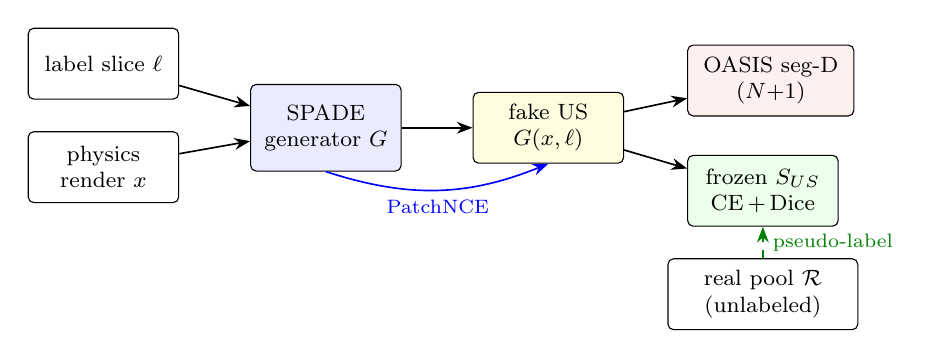
\begin{tikzpicture}[font=\footnotesize,
  box/.style={draw,rounded corners=2pt,align=center,inner sep=3pt,minimum height=9mm,text width=17mm},
  gen/.style={draw,fill=blue!8,rounded corners=2pt,align=center,inner sep=3pt,minimum height=11mm,text width=17mm},
  crit/.style={draw,fill=red!6,rounded corners=2pt,align=center,inner sep=3pt,minimum height=9mm,text width=19mm},
  arr/.style={-{Stealth[length=2mm]},line width=0.6pt}]
  \node[box] (label) {label slice $\ell$};
  \node[box,below=4mm of label] (phys) {physics render $x$};
  \node[gen,right=9mm of phys,yshift=5mm] (g) {SPADE\\generator $G$};
  \node[box,fill=yellow!12,right=9mm of g] (fake) {fake US\\$G(x,\ell)$};
  \node[crit,right=8mm of fake,yshift=6mm] (d) {OASIS seg-D\\$(N{+}1)$};
  \node[box,fill=green!8,right=8mm of fake,yshift=-8mm] (s) {frozen $S_{US}$\\CE\,+\,Dice};
  \draw[arr] (label) -- (g); \draw[arr] (phys) -- (g); \draw[arr] (g) -- (fake);
  \draw[arr] (fake) -- (d); \draw[arr] (fake) -- (s);
  \draw[arr,blue] (g.south) to[bend right=20] node[below,font=\scriptsize]{PatchNCE} (fake.south);
  \node[box,below=4mm of s,text width=22mm] (real) {real pool $\mathcal{R}$ (unlabeled)};
  \draw[arr,green!50!black,dashed] (real) -- (s.south) node[midway,right,font=\scriptsize]{pseudo-label};
\end{tikzpicture}}
\caption{SonoSPADE. The label slice and the physics render both condition the generator. A segmenter
$S_{US}$ pretrained free on aligned simulator pairs is frozen to pseudo-label the real pool for an
OASIS $(N{+}1)$ discriminator and to enforce a per-tissue consistency loss; PatchNCE preserves
content. No inverse generator, no cycle loss.}
\label{fig:pipeline}
\end{figure}

\subsection{Physics-conditioned dual-input generator}
$G$ is a ResNet encoder-decoder whose residual and upsampling blocks are SPADE-normalized: a
parameter-free instance norm whose per-pixel scale and bias are predicted from the resized label map
$\ell$, so the semantic layout modulates activations at every scale~\cite{park2019spade}. The
physics render $x$ is the content stream, so $G$ refines a tissue-correct render rather than
hallucinating anatomy. Content is preserved by multilayer PatchNCE on $G$'s own encoder
features~\cite{park2020cut} between $x$ and $G(x,\ell)$; there is no inverse generator and no cycle
loss.

\subsection{Free unpaired segmentation consistency}
The simulator emits perfectly aligned $(x,\ell)$ pairs, so a compact U-Net~\cite{ronneberger2015unet}
segmenter $S_{US}$ is pretrained at no annotation cost, then \emph{frozen} and used two ways. (i)~It
pseudo-labels the unlabeled real pool, giving an OASIS-style $(N{+}1)$-class per-pixel discriminator $D$
a semantic target for free~\cite{sushko2021oasis}: $G$ wins only when each synthesized pixel reads as
its conditioned tissue, a per-pixel realism signal. (ii)~A consistency loss
$\mathcal{L}_{seg}=\mathrm{CE}+\mathrm{Dice}$ requires $S_{US}(G(x,\ell))$ to match $\ell$, so $G$ cannot
collapse to a global recolor. The full objective is
\begin{equation}
\mathcal{L}=\mathcal{L}_{adv}^{\text{OASIS}}+\lambda_{nce}\mathcal{L}_{nce}
+\lambda_{seg}\mathcal{L}_{seg}+\lambda_{tc}\mathcal{L}_{tc},
\end{equation}
with class-balanced per-pixel cross entropy in $\mathcal{L}_{adv}$ so rare tissues are not ignored.

\subsection{Grouped scheme and training}
Fat, GI wall, pancreas, muscle, and generic soft tissue have near-equal backscatter and render
near-identically, so $S_{US}$ and $D$ operate in a \emph{grouped} scheme (these five merge; distinct
structures keep their class) while $G$ still conditions on the full $K$ classes. Three light stabilizers
help: a temporal-consistency term $\mathcal{L}_{tc}$ requiring $G$ to commute with a small in-plane
shift, an OASIS-style LabelMix on $D$~\cite{yun2019cutmix}, and an R1 gradient
penalty~\cite{mescheder2018r1} (average pooling keeps $D$ twice-differentiable); the deployed generator
is an EMA of the training weights.

\section{Experiments}
\subsection{Setup}
We build on a commodity-laptop ultrasound substrate that renders a physics B-mode from a CT-derived
canonical label volume (13 tissues via TotalSegmentator~\cite{wasserthal2023totalseg}) and exposes a
label-conditioned translator interface. Free aligned $(x,\ell)$ pairs come from eight abdominal CT
cases with pose sweeps and domain randomization. For the real head-to-head we use the public Kaggle
abdominal ultrasound set~\cite{vitale2020realism}: every translator is trained on its $404$-frame real
\emph{train} split, and evaluated on the disjoint $60$ annotated real frames (liver, kidney,
gallbladder, spleen, vessels), a leakage-free real test. All translators are evaluated on the same
held-out content. Everything runs on Apple Silicon (MPS, no CUDA).

\subsection{The label conditioning is genuinely per-tissue}
\label{sec:pertissue}
The central claim is that texture is per-tissue, not a global recolor. We measure this directly:
holding the physics render fixed, we relabel a tissue region and measure the texture change inside
versus outside. A global recolor scores near zero inside; SonoSPADE changes the region's own texture
$\inReg$ inside versus $\outReg$ outside (ratio ${\approx}\,13$), and the complementary label-swap
locality metric (Table~\ref{tab:main}) gives $\locSono$ versus $0$ for every label-free translator by
construction (Appendix Fig.~\ref{fig:qual}). Per-class speckle SNR also shifts per tissue, confirming
distinct learned statistics, not a uniform map.

\subsection{Free segmentation supervision}
$S_{US}$ pretrained on the aligned pairs reaches \liverDice{}/\lungDice{}/\vesselDice{} Dice on
liver/lung/vessels (acoustically distinct) on held-out patients. The canonical 13-class macro Dice is
capped at \diceCanon{} by degenerate soft tissues; merging them (grouped scheme) lifts it to \diceGroup{}
(merged soft-tissue class \softGroup{} vs \softCanon{}), with no change to distinct tissues --- an honest
reflection of B-mode acoustics, not a tuning artifact.

\subsection{Comparison to baselines}
\label{sec:baselines}
Table~\ref{tab:main} compares raw physics, CycleGAN~\cite{zhu2017cyclegan}, CUT~\cite{park2020cut}, an
S-CycleGAN-style variant~\cite{song2024scyclegan}, and SonoSPADE on the real Kaggle set.
\textbf{Structure:} SonoSPADE preserves anatomy far better than any learned translator (edge IoU
\iouSono{} vs \iouCUT{}/\iouCyc{} for CUT/CycleGAN, a $2.4\times$ margin) --- trained to match real
appearance, the tissue-agnostic translators aggressively remap the frame and drift on structure, while
physics-plus-label conditioning keeps anatomy intact. \textbf{Per-organ realism:} we report intensity
$W_1$ \emph{restricted to the annotated organ masks}, since the whole-frame score is dominated by the
background a global recolor matches trivially. Inside the masks the recolors' per-tissue fidelity
collapses (organ $W_1$ \wCyc{}/\wCUT{} vs \wPhys{} for the render they started from), whereas SonoSPADE
keeps it (\wSono{}, ${\approx}\,2\times$ better than any learned baseline and closest to raw physics),
and is the only method with per-tissue control (locality \locSono{} vs $0$). \textbf{TSTR} is near zero
for all linear methods (SonoSPADE lowest, \tstrSono{}; kidney/spleen Dice $0$): the score is dominated
by the linear-vs-curvilinear geometry gap no method addresses, and is further depressed for SonoSPADE
because its conditioning shifts features from what the pretrained classifier expects. Matching the
sector geometry and adding test-time adaptation resolves most of it and reverses the ranking (next).

\begin{table}[t]
\centering
\caption{Baseline comparison on the real Kaggle set. Edge IoU (structure vs the physics input, higher
better); \emph{organ} intensity $W_1$ (mean over the five annotated organs, excluding the background a
global recolor trivially matches; lower better); label-swap locality (per-tissue control, higher
better; $0$ for label-free translators by construction); and TSTR Dice. SonoSPADE preserves structure
$2.4\times$ better than the best baseline and per-organ intensity roughly $2\times$ better than any
learned translator, and is the only method with per-tissue control. TSTR is near zero for all linear
methods, dominated by the sim-to-clinical geometry gap (see text); the SonoSPADE-curvi row renders the
same content in the matched sector geometry (Experiment~A, Sec.~\ref{sec:tstr}), and its TSTR is the
five-seed mean from Table~\ref{tab:tstr}.}
\label{tab:main}
\begin{tabular}{lcccc}
\toprule
Method & Edge IoU $\uparrow$ & Organ $W_1$ $\downarrow$ & Locality $\uparrow$ & TSTR Dice $\uparrow$\\
\midrule
Raw physics            & \iouPhys & \wPhys  & \locPhys & \tstrPhys\\
CycleGAN               & \iouCyc  & \wCyc   & \locCyc  & \tstrCyc\\
CUT                    & \iouCUT  & \wCUT   & \locCUT  & \tstrCUT\\
S-CycleGAN (reimpl.)   & \iouSCyc & \wSCyc  & \locSCyc & \tstrSCyc\\
\textbf{SonoSPADE}     & \iouSono & \wSono  & \locSono & \tstrSono\\
\midrule
SonoSPADE-curvi        & \iouSonoCurvi & \wSonoCurvi & \locSonoCurvi & \tstrSonoCurvi\\
\bottomrule
\end{tabular}
\end{table}

\paragraph{Whole-frame realism (FID/KID).} SonoSPADE does \emph{not} win whole-frame FID/KID (Appendix
Table~\ref{tab:fidkid}): its scores sit near the untranslated render and above the tissue-agnostic
translators. This is the organ-$W_1$ story from the other side --- FID/KID score \emph{overall}
appearance, which a global tone map matches cheaply and which is blind to whether each organ reads
correctly. Matching the sector geometry improves all absolute scores (a large confound) but not the
ranking; SonoSPADE's advantage is per-organ fidelity and per-tissue control, and we do not optimize FID.

\subsection{Ablation of the training terms}
Ablating SonoSPADE's terms one at a time (retrained at a fixed shared budget; Appendix
Table~\ref{tab:abl}) shows the segmentation-consistency term is the largest single contributor: removing
it roughly halves label-swap locality (\ablLocFull{} to \ablLocSeg{}) and degrades structure (edge IoU
\ablIouFull{} to \ablIouSeg{}) and per-organ $W_1$ (\ablWFull{} to \ablWSeg{}). Locality does not fall to
a label-free translator's zero --- SPADE injects the label at every scale --- but the explicit
consistency term is what roughly doubles it. Dropping the OASIS LabelMix or the temporal term leaves
per-frame fidelity unchanged (their roles are discriminator regularization and frame-to-frame stability).

\subsection{Closing the sim-to-real gap for downstream transfer}
\label{sec:tstr}
The near-zero TSTR of Table~\ref{tab:main} is a geometry problem, not texture: our substrate renders a
\emph{linear} rectangular frame while Kaggle frames are \emph{curvilinear} sector scans, so a segmenter
trained on the linear render meets a different spatial prior at test time. Two drop-in fixes
(Table~\ref{tab:tstr}). \textbf{(A)}~A curvilinear remap warps the (image, label) render into the
measured sector geometry (${\approx}\,44^{\circ}$; Appendix Fig.~\ref{fig:qual}) at train and inference,
plus probe-motion augmentation: TSTR rises ${\approx}\,4\times$ for SonoSPADE and ${\approx}\,2\times$
for the raw render, tying them (\tstrSonoCurvi{}$\pm$\tstrSonoCurviSd{} vs
\tstrPhysCurvi{}$\pm$\tstrPhysCurviSd{}, \ttaSeeds{} seeds) --- geometry alone moves SonoSPADE from worst
to on par. \textbf{(B)}~Test-time adaptation (TENT) of the downstream segmenter's BatchNorm affine on
$50$ unlabeled real frames raises SonoSPADE to \tstrSonoTent{} but the raw render only to \tstrPhysTent{}
(about $3\times$ the gain, because realistic texture makes the synthetic feature statistics adaptable),
so SonoSPADE \emph{overtakes} on every one of the \ttaSeeds{} seeds. Absolute Dice stays low (kidney and
spleen hard, $60$-frame test), so this is directional evidence that texture aids transfer once geometry
is matched, not clinical-grade segmentation.

\begin{table}[t]
\centering
\caption{Downstream transfer (TSTR Dice, higher better) as geometry and test-time adaptation are added.
Curvilinear and TENT numbers are the mean $\pm$ std over \ttaSeeds{} downstream seeds; the linear row is
the single deployed run of Table~\ref{tab:main}. Geometry (A) brings SonoSPADE from worst to tied with
the raw render; TENT (B) makes it overtake, on every seed.}
\label{tab:tstr}
\begin{tabular}{lcc}
\toprule
Setting & Raw physics $\uparrow$ & SonoSPADE $\uparrow$\\
\midrule
Linear render (Table~\ref{tab:main})   & \tstrPhys & \tstrSono\\
$+$ curvilinear remap (A)              & \tstrPhysCurvi{} {\footnotesize $\pm$\tstrPhysCurviSd} & \tstrSonoCurvi{} {\footnotesize $\pm$\tstrSonoCurviSd}\\
$+$ curvilinear $+$ TENT (B)           & \tstrPhysTent{} {\footnotesize $\pm$\tstrPhysTentSd} & \textbf{\tstrSonoTent}{} {\footnotesize $\pm$\tstrSonoTentSd}\\
\bottomrule
\end{tabular}
\end{table}

\subsection{Inference latency: real time, no GPU}
\label{sec:latency}
The texture stage is built to run inside a reinforcement-learning acquisition loop, so per-frame
latency, not peak realism, is the binding constraint. A single generator pass takes $66$\,ms on CPU
($15$ frames/s) and $12$\,ms on an integrated GPU ($85$ frames/s) at batch one, with \emph{no discrete
GPU} (measured, \texttt{scripts/bench\_latency.py}). A semantic-diffusion synthesizer of higher realism
instead runs $T$ denoising passes per frame. Measured on the same machine, a representative ADM/SDM-style
denoising U-Net (the family Echo-from-noise~\cite{stojanovski2023echofromnoise} builds on; $62$M
parameters, sized conservatively so it lower-bounds the diffusion cost, and latency is architecture- and
step-count-bound, not weight-bound) costs $186$\,ms/pass on CPU and $26$\,ms on the integrated GPU ---
only ${\approx}\,2.7\times$ a SonoSPADE pass, but its $T$ passes make it two orders of magnitude slower
\emph{per frame} at a standard $T{=}50$ ($133\times$ CPU) and up to three at full DDPM ($T{=}250$--$1000$),
narrowing to ${\approx}\,66\times$ only under aggressive $25$-step DDIM.
For a loop of millions of frames, seconds per frame is prohibitive. We cede the whole-frame FID/KID crown
for this real-time, GPU-free inference; the realism-first
methods~\cite{vitale2025realism,stojanovski2023echofromnoise} target offline augmentation where seconds
per frame is acceptable, and unlike the equally-fast tissue-agnostic baselines SonoSPADE is per-tissue.
We verified this \emph{in situ}: SonoSPADE runs inside a MuJoCo closed-loop ultrasound-acquisition environment,
where an imitation-warm-started REINFORCE policy trains and executes against it, rendering a fresh
textured frame at every agent step on held-out patients without the texture stage becoming the
bottleneck. This is an integration-and-throughput result; the effect on \emph{acquisition quality} is
the subject of Sec.~\ref{sec:organrl}.

\subsection{Per-tissue texture improves an in-the-loop acquisition agent}
\label{sec:organrl}
The latency result says the texture stage \emph{can} run in the loop; it does not say per-tissue texture
\emph{helps} the agent. Showing that needs a task whose reward depends on per-tissue correctness, scored
by a judge that is \emph{fixed across} texture stages rather than matched to each (the flaw that made our
earlier goal-reaching benchmark uninformative, Sec.~\ref{sec:limitations}). We build one:
\emph{organ-conditioned acquisition}. A probe starts with the target organ partially in view and servos
to bring it in; the per-step reward is the confidence of a frozen organ recognizer $J$ that the organ is
present in the current textured frame. $J$ is trained \emph{only on real} Kaggle frames and masks (never
on simulator or SonoSPADE output, so the reward is non-circular) and is the \emph{same} $J$ for every
texture stage. The primary metric is texture-independent: the ground-truth fraction of the acquired view
that is the target organ, from the true label slice.

First, is the reward viable, i.e.\ does $J$ recognize the correct organ better under SonoSPADE than under
a global recolor? On held-out simulator content $J$'s liver IoU is \recSono{} for SonoSPADE versus
\recCut{} (CUT) and \recCyc{} (CycleGAN) under a border-cropped $J$ domain-matched to the borderless sim
render ($0.27$ vs $0.07$--$0.21$ under a full-frame $J$; the ordering is robust to that choice),
approaching the real-data ceiling \recCeil{} (Table~\ref{tab:organrl}, \rlSeeds{} seeds; the lead holds
on precision too, so it is not a liver-flooding artifact). Notably the untranslated render itself scores
\recPhys{}, \emph{above} both recolors: the global recolors actively degrade liver recognition, while
SonoSPADE improves on the render --- so part of the effect is structure preservation (SonoSPADE also
keeps anatomy best, edge IoU in Table~\ref{tab:main}), not per-tissue texture alone. A fair comparison
also requires all three translators trained on the \emph{same} real pool; scoring CUT with an off-pool
checkpoint spuriously reverses the result --- a reproducibility pitfall we flag and fix. Trained under
this reward (imitation-warm-started REINFORCE, \rlSeeds{} seeds, held-out patients), SonoSPADE reaches
the highest ground-truth liver visibility, $\rlSono\,{\pm}\,\rlSonoSd$, above CUT (\rlCut{}), CycleGAN
(\rlCyc{}) and the untranslated render (\rlPhys{}) from a static start of \rlStart{}, with all three
per-seed paired differences positive ($+0.003$ to $+0.015$; sign-consistent across \rlSeeds{} seeds, so
directional rather than significance-tested). Its reward signal is roughly twice as strong (\rewSono{}
vs \rewCut{}--\rewPhys{}), but the ground-truth margin is \emph{small}: the imitation warm-start and
liver's dominance already nearly solve the task. This is a modest, seed-consistent positive --- to our
knowledge the first evidence that per-tissue texture helps an in-the-loop agent under a fixed external,
real-trained judge.

The effect is confined to liver: for kidney, spleen and gallbladder \emph{no} translator (SonoSPADE
included) yields a rendering the recognizer identifies (IoU ${\approx}\,0$), even rendered prominently
with $J$ rebalanced --- the same $J$ scores them $0.3$--$0.8$ on \emph{real} data. The bottleneck is the
simulator-plus-translator's failure to reproduce their real appearance (kidney lacks cortico-medullary
structure; spleen is acoustically near-identical to liver; the anechoic gallbladder is brightened), not
the recognizer, so the multi-organ per-tissue claim rests on the offline metrics (locality, organ-$W_1$)
and the in-the-loop gain is shown for the one organ that transfers.

\begin{table}[t]
\centering
\caption{Organ-conditioned liver acquisition (\rlSeeds{} seeds, held-out patients). Top: a real-trained
recognizer $J$ (fixed across texture stages) recognizes SonoSPADE's liver far better than a global
recolor's (liver IoU; real-data ceiling \recCeil{}). Middle: trained under $J$'s confidence as reward,
SonoSPADE reaches the highest \emph{ground-truth} liver visibility (true label, texture-independent;
static start \rlStart{}), higher in \rlSeeds{}/\rlSeeds{} seeds. Bottom: SonoSPADE's reward signal is
${\sim}2\times$ stronger. Harness and the CUT-checkpoint fairness fix in \texttt{scripts/premise/}.}
\label{tab:organrl}
\begin{tabular}{lcccc}
\toprule
 & physics & CUT & CycleGAN & SonoSPADE\\
\midrule
$J$ liver recognition, IoU $\uparrow$        & \recPhys{} & \recCut{} & \recCyc{} & \textbf{\recSono{}}\\
Ground-truth liver acquired $\uparrow$       & \rlPhys{}  & \rlCut{}  & \rlCyc{}  & \textbf{\rlSono{}}\\
Reward signal ($J$ conf., secondary) $\uparrow$ & \rewPhys{} & \rewCut{} & \rewCyc{} & \textbf{\rewSono{}}\\
\bottomrule
\end{tabular}
\end{table}

\section{Limitations}
\label{sec:limitations}
Unpaired training matches per-tissue statistics, not exact speckle: the output is training texture, not
diagnostic imagery. Acoustically similar soft tissues are near-inseparable in B-mode, so per-tissue
fidelity is strong only for distinct structures. Validation is on a \emph{single} dataset and anatomy
(abdominal Kaggle, $60$ annotated real frames, $8$ CT cases); external validity to other anatomies and
scanners is untested, and the downstream Dice stays low even after the geometry+TENT fixes (kidney and
spleen barely transfer), so the transfer result is directional, not clinical-grade. A larger,
multi-anatomy matched-view clinical set is the honest next step.

Our evidence that SonoSPADE \emph{improves} an agent is real but bounded. It does not come from the
earlier goal-reaching benchmark, whose per-texture \emph{matched} judge is not comparable across texture
stages (a random policy scores ${\approx}\,0.36$ under one judge versus ${\approx}\,0.03$ under another);
the organ-conditioned task of Sec.~\ref{sec:organrl} fixes that but the gain is small, seed-consistent
rather than significance-tested (\rlSeeds{} seeds), and liver-only. A harder, less liver-dominated
target and a translator that reproduces smaller-organ appearance is the next step to a larger effect.

\section{Conclusion}
SonoSPADE is a real-time, GPU-free, per-tissue ultrasound texture stage for closed-loop acquisition:
conditioning on both a physics render and the tissue label slice makes texture per-tissue and
controllable, and a segmenter pretrained free on simulator pairs supplies discriminator supervision and
a consistency signal with no paired real labels. A label-swap locality metric quantifies that the
conditioning is genuinely per-tissue (${\approx}\,\locality$ versus $0$ for label-free translators),
addressing a stated evaluation gap. Matching the clinical sector geometry and adapting the downstream
segmenter at test time turn a near-zero transfer into SonoSPADE overtaking the untranslated render on
every seed, and on an organ-conditioned acquisition task scored by a fixed real-trained recognizer the
per-tissue reward gives the highest ground-truth liver visibility in all three seeds --- a small,
liver-only in-the-loop proof of concept. The whole method trains on a commodity laptop.

\paragraph{When to use it.} SonoSPADE is for controllable, label-consistent synthetic data without real
annotations: because texture is conditioned on the label, the frame and its mask stay aligned, whereas a
global recolor scrambles the per-tissue statistics the labels describe. The recipe and the locality
metric transfer to any modality with an aligned-pair simulator. When photorealism alone is the goal a
global translator remains the better choice --- SonoSPADE is for trustworthy labeled data with
per-tissue appearance, not the most realistic single image.

\bibliographystyle{splncs04}
\bibliography{references}

\appendix
\section{Appendix: supplementary tables and figures}
\label{sec:appendix}

\begin{table}[h]
\centering
\caption{Whole-frame FID/KID ($\times 10^{3}$) against the real pool (InceptionV3), lower better.
SonoSPADE is not competitive by design (these reward the global recolor it does not perform); the
bottom block re-runs in the sector geometry, improving all absolute scores but not the ranking.}
\label{tab:fidkid}
\begin{tabular}{lcc}
\toprule
Method & FID $\downarrow$ & KID $\times 10^{3}$ $\downarrow$\\
\midrule
Raw physics            & \fidPhys & \kidPhys\\
CycleGAN               & \fidCyc  & \kidCyc\\
CUT                    & \fidCUT  & \kidCUT\\
S-CycleGAN (reimpl.)   & \fidSCyc & \kidSCyc\\
SonoSPADE              & \fidSono & \kidSono\\
\midrule
Raw physics-curvi      & \fidPhysCurvi  & \kidPhysCurvi\\
CycleGAN-curvi         & \fidCycCurvi   & \kidCycCurvi\\
CUT-curvi              & \fidCUTCurvi   & \kidCUTCurvi\\
S-CycleGAN-curvi       & \fidSCycCurvi  & \kidSCycCurvi\\
SonoSPADE-curvi        & \fidSonoCurvi  & \kidSonoCurvi\\
\bottomrule
\end{tabular}
\end{table}

\begin{table}[h]
\centering
\caption{Ablation (one term off per row; retrained at a fixed budget). Removing the frozen $S_{US}$
seg-consistency term roughly halves locality and degrades structure --- the largest single effect.}
\label{tab:abl}
\begin{tabular}{lccc}
\toprule
Variant & Edge IoU $\uparrow$ & Organ $W_1$ $\downarrow$ & Locality $\uparrow$\\
\midrule
Full SonoSPADE          & \ablIouFull & \ablWFull & \ablLocFull\\
$-$ $S_{US}$ consistency & \ablIouSeg  & \ablWSeg  & \ablLocSeg\\
$-$ OASIS LabelMix       & \ablIouLm   & \ablWLm   & \ablLocLm\\
$-$ temporal consistency & \ablIouTc   & \ablWTc   & \ablLocTc\\
\bottomrule
\end{tabular}
\end{table}

\begin{figure}[h]
\centering
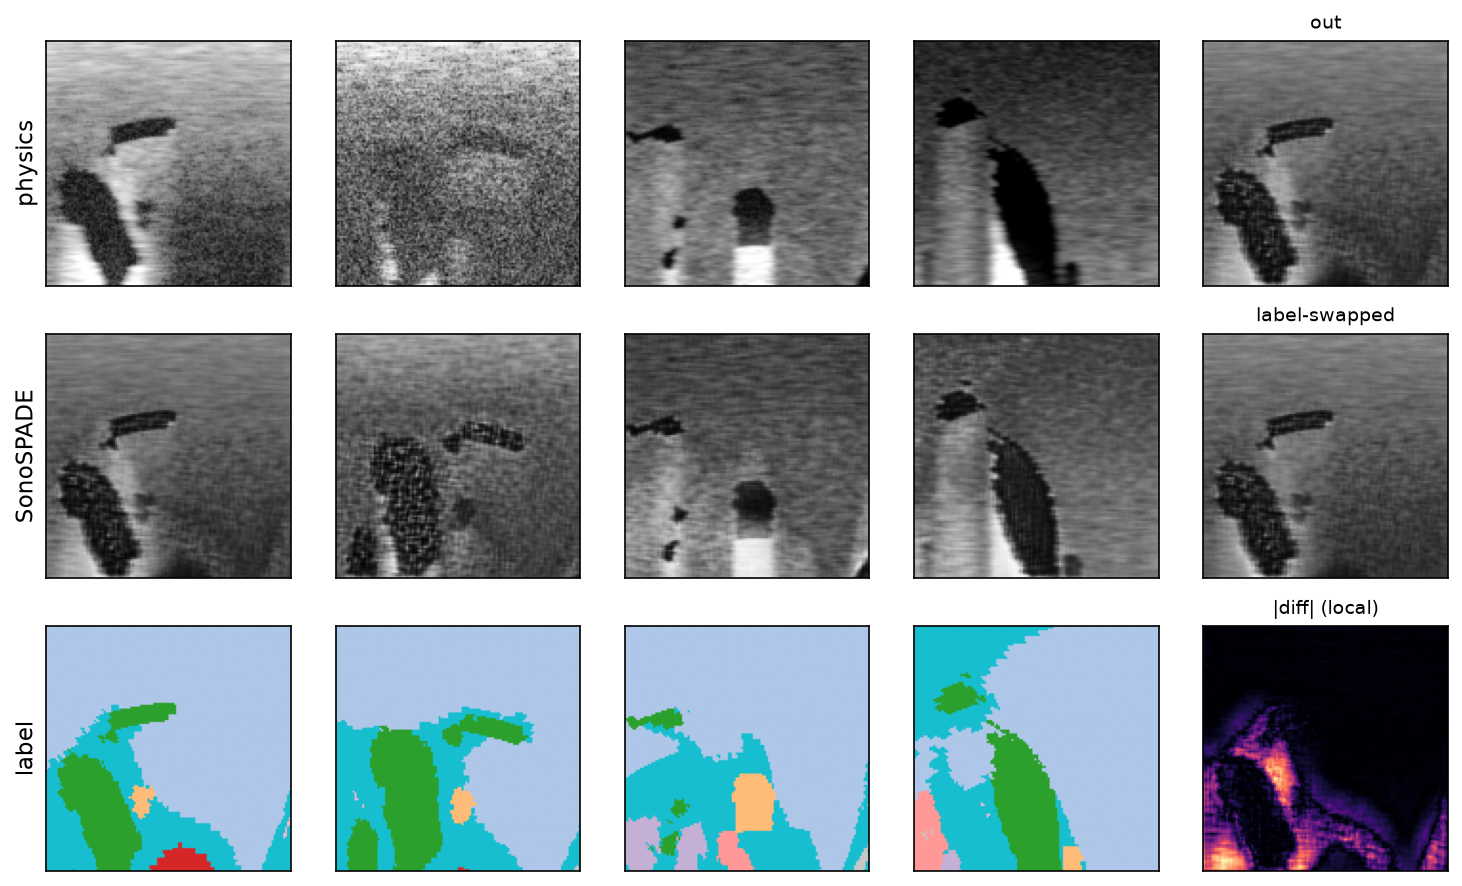
\includegraphics[width=0.62\linewidth]{qualitative.png}\hfill
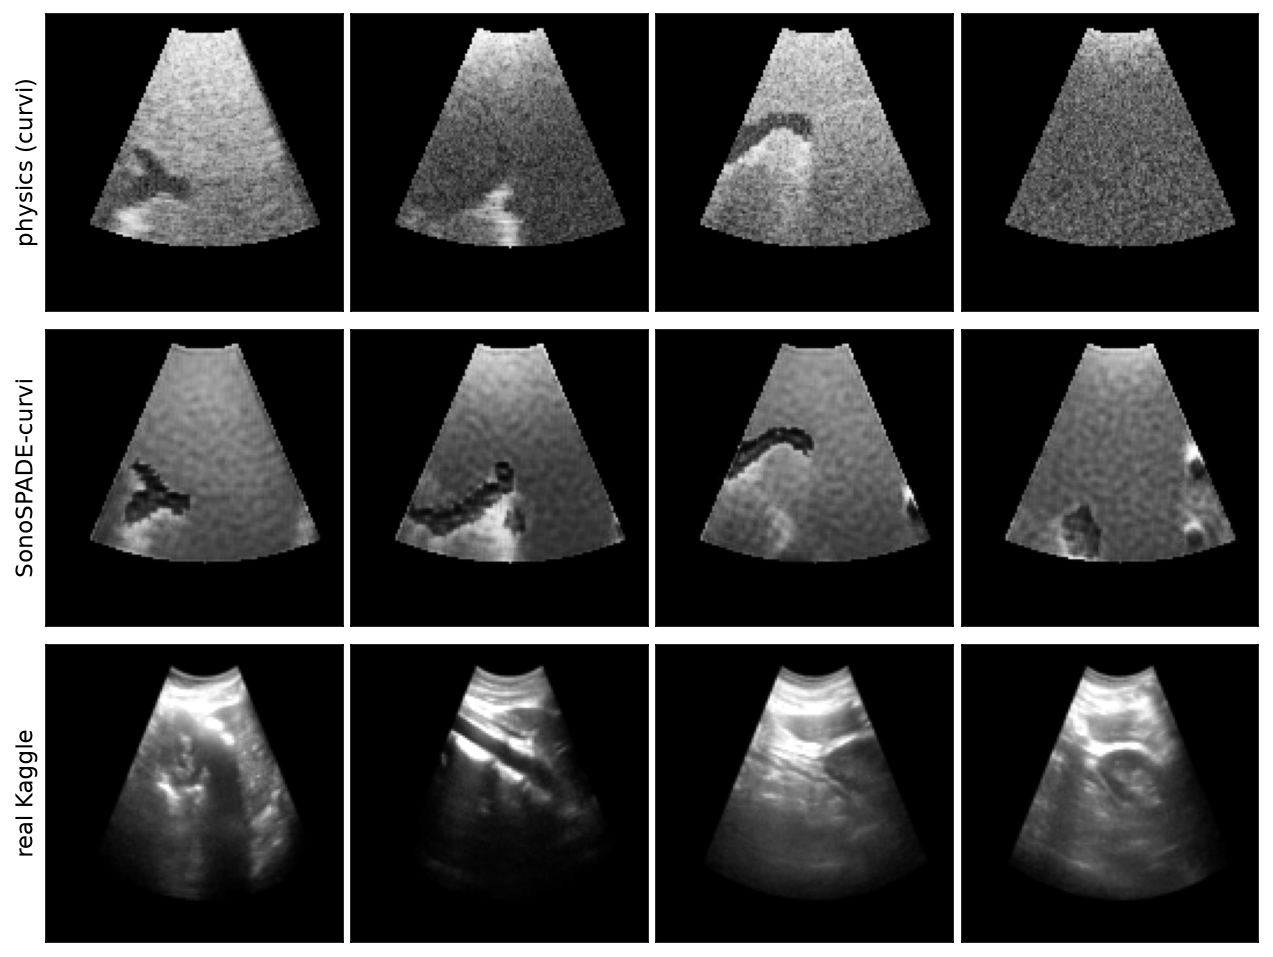
\includegraphics[width=0.36\linewidth]{figures/curvilinear.png}
\caption{Left, per-tissue qualitative result (Sec.~\ref{sec:pertissue}): physics render, SonoSPADE
output, tissue label (rows); each tissue gets its own speckle, and relabeling a region changes its
texture locally. Right, Experiment~A (Sec.~\ref{sec:tstr}): after the curvilinear remap the curvilinear
physics render (top), SonoSPADE-curvi (middle), and a real Kaggle frame (bottom) share the sector field.}
\label{fig:qual}
\end{figure}

\end{document}
